%************************************************
\chapter{The effects of alignment error and alignment filtering on the sitewise detection of positive selection}
\label{ch_indels1}
\acresetall
%************************************************

\section{Introduction}



The decreasing cost of DNA sequencing has triggered a striking
increase in the number of model and non-model organisms with planned
genome sequencing projects, suggesting that the range and scale of
comparative genomics applications will continue to expand
\citep{Green2007,Birney2007}. The existence of clusters of
closely-related genome sequences across a wide taxonomic range has led
to a better understanding of which aspects of molecular evolution are
variable and which are constant \citep{Wolf2009Nonlinear}, and an
increased sampling of species should continue to boost the power and
accuracy of individual analyses within a given clade.

The study of protein evolutionary rates and selective pressures in
particular has flourished as a result of the growth in comparative
genomic datasets. This is especially beneficial for the calculation of
spatially precise evolutionary estimates, as additional species
sampling has been shown to be an effective means of boosting the
accuracy and power of \sw detection of positive selection and
evolutionary constraint
\citep{Anisimova2001,Massingham2005}. Site-specific
evolutionary estimates have proved especially valuable when analyzed
in conjunction with other protein-based datasets such as structural
features \citep{Lin2007Proportion,Ramsey2011Relationship}, human
population diversity \citep{2010Map} and human disease mutations
\citep{Arbiza2006Selective}.

A major concern in the detection of positive selection in proteins is
that the effect of alignment error is not well
characterized. Intuitively, one might expect alignment error to result
mainly in an increased number of false positives, as the spurious
alignment of \nh codons on average would result in a high number of
apparent \nsyn substitutions and a low number of \syn substitutions
(since two randomly chosen codons are more likely to be \nsyn than
\syn).  However, false negatives may also be introduced, either
through the introduction of \syn but \nh codons into a
positively-selected site (thus reducing power due to an inflated \syn
substitution rate) or through the failure to align truly homologous
codons at a positively-selected site (reducing power due to less
evidence for positive selection at that site).  Since different
aligners employ a variety of algorithms, evolutionary models, and
heuristic optimizations \citep{Notredame2007Recent}, each program may
be more or less prone to different types of alignment error, causing
potentially large variations in the nature and magnitude of its impact
on the detection of positive selection. Different aligners may also be
designed for different downstream applications, such as phylogenetic
inference or functional annotation \citep{Morrison2009}, making the
optimal choice of aligner potentially dependent on the way in which
the resulting alignment will be used. This chapter focuses on methods
for the sitewise detection of positive selection, as they will be be
widely used throughout this thesis.
%In this chapter, I focused on
%the sitewise detection of positive selection.
 
In addition to the choice of aligner, the protein structure and
evolutionary divergence of a dataset may contribute to the effects of
alignment error. Differently structured protein regions show variable
tolerance to biological indels, with indels more common in
extracellular and transmembrane proteins than in highly folded enzymes
and housekeeping genes \citep{delaChaux2007DNA}. This suggests that
well-folded protein regions will experience fewer biological
indels---and will therefore be less susceptible to alignment
error---than less structured regions.

The evolutionary divergence of a dataset affects the power of \sw
inference and the prevalence of indels in multiple ways. As
maximum-likelihood methods for detecting positive selection require
data in the form of fixed substitutions between species, they show
little power at low divergence and their highest power at intermediate
to high divergence levels \citep{Anisimova2001}. However, alignment
error should be greatest at high divergences, which may have the
effect of reducing power. These two trends suggest that the overall
power will be low at both extremes of divergence, with little
inference power at low divergence (due to the scarcity of data in the
form of observed substitutions) and an overwhelming amount of
alignment error at high divergence (due to the large number of indel
events).

Fortunately, the majority of genes in many biological clades of
interest (such as mammals, vertebrates, fruit flies, and yeast) fall
within the middle range of divergences where \sw methods are at their
most powerful and where multiple alignment is a difficult---but not
hopeless---problem. As such, it is important to seek an understanding
of the impact of alignment error on overall error rates within this
important range of divergence levels.

A number of empirical analyses have established that errors in gene
sequencing, annotation and alignment can contribute to errors in
downstream evolutionary analyses such as phylogeny inference
\citep{Wong2008Alignment} and estimates of positive selection
\citep{Schneider2009,MarkovaRaina2011}. Most recently,
\citet{MarkovaRaina2011} showed
that the detection of positively-selected sites and genes in \Dr
genomes is highly sensitive to aligner choice, with PRANK's codon
model \citep{Loytynoja2008PhylogenyAware} consistently producing
alignments with the lowest amount of positive selection. Still,
according to the authors' manual inspection of alignments, even
positively-selected sites identified with PRANK alignments contained a
sizable proportion of apparent false positives.

A limitation of the analysis of error in empirical datasets is the
lack of a benchmark set of true alignments and positively-selected
sites. \citet{MarkovaRaina2011} used their expected general effect of
alignment error (an increase in false positives due to misalignment of
non-homologous codons) as a proxy by which to compare different
methods, allowing for the conclusion that PRANK was the least
error-prone aligner in their analysis. However, the absolute number of
false positives remained uncertain and there was the possibility of
conflating multiple sources of error: in addition to alignment error,
the authors noted that gene mis-annotation was responsible for many
apparent false positives, and there is also an expected error rate
from the likelihood inference method itself. This limitation leaves
important and interesting questions, regarding the nature of alignment
error and its quantitative impact on the detection of positive
selection, unanswered by empirical studies.

Controlled simulation experiments provide a natural framework for
investigating error rates in detail, allowing one to pinpoint the
sources of error in multi-step analyses such as alignment followed by
evolutionary inference. This approach has been employed in assessing
the robustness of phylogenetic inference methods to misalignment
\citep{Dwivedi2009Phylogenetic,Ogden2006Multiple,Loytynoja2008PhylogenyAware},
but those results cannot be easily extrapolated to the analysis of \sw
selective pressures. More recently, \citet{Fletcher2010} performed a
series of simulation experiments investigating alignment error in the
use of the branch-site test to detect positive selection in
genes. Their results showed that most aligners caused false positives
by over-aligning codons and that datasets from mammalian and
vertebrate gene families contain enough evolutionary divergence to
make false positive errors resulting from misalignment a legitimate
concern.

Reflecting a widespread awareness of the problem of misalignment,
methods for identifying and removing uncertain or unreliable alignment
regions have been commonly used in phylogenetic and molecular
evolutionary analyses. The popular Gblocks program applies a set of
heuristic criteria to identify conserved blocks deemed suitable for
phylogenetic or evolutionary analysis \citep{Castresana2000Selection}
while a number of aligners such as T-Coffee
\citep{Notredame2000} and PRANK
\citep{Loytynoja2008PhylogenyAware} produce estimates of alignment
confidence or reliability. GUIDANCE, which measures the robustness of
alignment regions to perturbations in the guide tree used for
progressive alignment, has also been proposed as an alignment
confidence score \citep{Penn2010Alignment}. Unfortunately, despite
their widespread use, the impact of the many available alignment
scoring and filtering methods on phylogenetic and evolutionary
analyses has not been well studied. Even for a single filtering
program, Gblocks, results have been contradictory: one
simulation-based study found that it improved the phylogenetic signal
\citep{Talavera2007Improvement} while an empirical study across a wide
range of taxa found that Gblocks-filtered alignments produced worse
phylogenetic trees than unfiltered alignments
\citep{Dessimoz2010Phylogenetic}. A recent study using a variety of
filters suggested that the benefit of alignment filtering (in terms of
improved accuracy) outweighs the cost (in terms of reduced power) when
applied to detecting positive selection \citep{Privman2011Improving},
but this analysis was limited to a small range of possible
evolutionary scenarios as discussed below.  With the application of
published filtering methods to alignments before testing for positive
selection becoming standard practice
\citep{Studer2008,Aguileta2009Rapidly}, continued
investigation of potential benefits of alignment filtering to the
detection of positive selection seems well-warranted.

This chapter aims to use a simulation framework to incorporate
alignment error and alignment filtering into estimates of the error
rate and power of \sw evolutionary inference of positive
selection. This approach builds on those of \citet{Anisimova2002},
\citet{Fletcher2010}, and \citet{Privman2011Improving}, using
simulated protein alignments including insertions and deletions to
evaluate methods for detecting \sw positive selection. Furthermore, a
diverse sample of aligners and alignment filters were incorporated
into an experimental design that differs from previous ones in a
number of important ways.

I focused on sitewise detection of positive selection occurring
throughout a phylogeny and evaluated the impact of a number of
alignment filtering methods on the \sw analysis. Thus, the biological
hypothesis being investigated was different from that studied by
\citet{Fletcher2010}, who focused on genewise selection acting at
specific branches.  \citet{Privman2011Improving} recently published a
related paper considering the evolutionary characteristics of three
HIV-1 genes. They concluded that alignment filtering improves the
performance of positive selection inference by reducing false positive
results. While this may be true for these three genes (and perhaps for
HIV-1 in general), HIV-1 is known to evolve with widespread positive
selection in the human host \citep{Yang2003Widespread}. Results valid
for these genes may not be widely applicable to large-scale vertebrate
and mammalian comparative datasets, which exhibit less adaptive
evolution \citep{Kosiol2008} and which comprise a larger diversity of
protein structures and a wider range of species divergence levels.

I hypothesized that the divergence level and indel rate---two important
evolutionary factors which are highly variable within and between
different genomes---may strongly affect the performance of methods for
alignment and detection of selection. Accordingly, these simulations
encompassed a wide range of biologically plausible indel rates and
divergence levels while fixing other parameters at values typical to
those encountered in the \sw analysis of vertebrate gene families.

\section{Methods}


\bbtable
\centering
\begin{tabular}{lllllllll}
\toprule
 \multicolumn{3}{c}{Tree} & \multicolumn{3}{c}{Insertions and Deletions} & \multicolumn{3}{c}{$\omega$ Distribution} \\
\cmidrule(r){1-3} \cmidrule(r){4-6} \cmidrule(r){7-9}
 & & &  & Mean Length & & & & \\
Taxa & Source & MPL & Size Distribution & (Std. Dev.) & Rate & Shape & Mean & $p (\omega>1)$ \\
\midrule
6 & Artificial & & power law & & & lognormal & & \\
17 & $\beta$-globin & 0.05--2.0 & decay: 1.8 & 3.33 (5.51) & 0--0.2 & log mean: -1.864 & 0.277 & 0.06 \\
44 & Vertebrates & & max length: 40 & & &  log SD: 1.201 & & \\
\bottomrule
\end{tabular}
\caption{Parameter Values Used in Simulations. \ac{mpl} is the mean
  path length of the tree in units of substitutions per synonymous
  site (\ds). Indel lengths are measured in units of codons, and the
  indel rate is defined as the number of insertion \& deletion events
  per substitution.}
\label{table_indels_1}
\eetable

\subsection{Alignment Simulations}

An overview of the simulation parameters used in this study can be
found in Table \ref{table_indels_1}. Three rooted trees were used to
guide the simulation of protein-coding DNA alignments: the artificial
6-taxon tree used by \citet{Anisimova2001} and
\citet{Massingham2005} rooted at its midpoint, the 17-taxon
vertebrate $\beta$-globin tree from \citet{Yang2000CodonSubstitution}
and the 44-taxon vertebrate tree used by the ENCODE project
\citep{Birney2007,Nikolaev2007}. Trees, shown with their original
branch lengths in Figure \ref{fig_1}, were scaled to comparable
divergence levels by normalizing their mean path length (MPL), defined
as the root-to-tip branch length averaged across all lineages in the
tree. I simulated alignments with MPL divergence between 0.05 and 2.0
\syn substitutions per \syn site, spanning the range of evolutionary
divergences observed in several clades of organisms with
fully-sequenced genomes (Table \ref{table_2}).

\begin{figure}[t!]
\centering
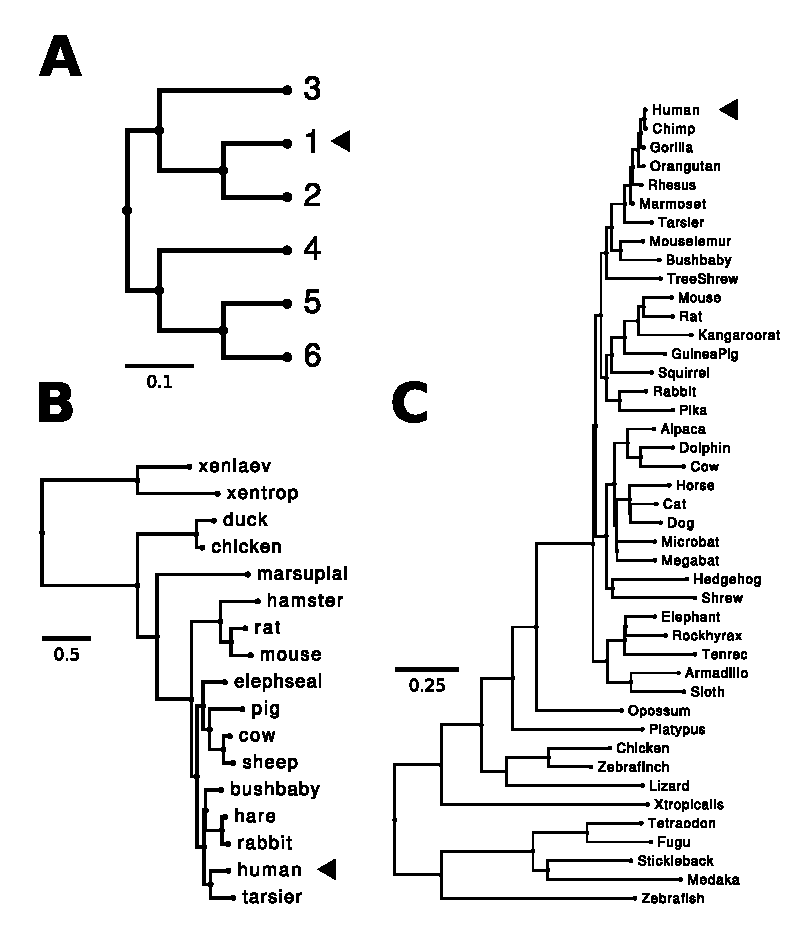
\includegraphics[scale=0.6]{Figs/fig1.pdf}
\caption{Phylogenetic trees used for simulation and analysis. The
  original scale for each tree is indicated by a scale bar, but trees
  were scaled to equal mean path length (MPL) divergence levels for
  simulation. (A) A 6-taxon artificial tree used in previous
  simulations
  \citep{Anisimova2001,Massingham2005}. (B) A tree
  estimated from $\beta$-globin genes of 17 vertebrates and used in
  previous empirical analyses and simulation studies
  \citep{Anisimova2001,Anisimova2002}. (C) The
  44-species tree used by the ENCODE project
  \citep{Birney2007,Nikolaev2007}. The nodes indicated by
  arrows were used as the reference species when comparing the true
  and inferred alignment (see Methods).}
\label{fig_1}
\end{figure}


\begin{table}
\centering
\begin{tabular}{lrrl}
\toprule
 Species & Pairwise $dS$ & Root-to-tip $dS$ & Reference \\
\midrule
   Human-Chimp & 0.01 & (0.005) & \citealp{Nei2010Neutral}
\\ Human-Mouse & 0.43 & (0.215) & \citealp{Nei2010Neutral}
\\ Human-Mouse & 0.5 - 0.8 & (0.25 - 0.4) & \citealp{Ogurtsov2004Indel}
\\ Human-Chicken & 0.9 & (0.45) & \citealp{Nei2010Neutral}
\\ Human-Chicken & 1.66 & (0.83) & \citealp{Hillier2004}
\\ Human-Zebrafish & 1.38 & (0.69) & \citealp{Nei2010Neutral}
\\ Vertebrates & -- & 0.75 & \citealp{Siepel2005}
\\ Drosophila & -- & 1.0 & \citealp{Siepel2005}
\\ Yeasts & -- & 1.25 & \citealp{Siepel2005} \\
\bottomrule
\end{tabular}
\caption{Genome-wide Divergence Estimates for Commonly Analyzed
  Eukaryotes. The root-to-tip $dS$ is equivalent to the MPL (mean path
  length) used in these simulations. For two-species comparisons where
  the pairwise $dS$ was given, the root-to-tip $dS$ was calculated as
  half of the pairwise $dS$ and is included in parentheses.}
\label{table_2}
\end{table}

The INDELible program \citep{Fletcher2009INDELible} was used to
simulate codon sequences with indels along each phylogenetic tree. The
length of the root sequence was set to 500 codons and $\bm{\kappa}$ (the
ratio of transition to transversion substitutions) was fixed at 4.
Indel lengths were drawn from a discretized
power-law distribution with an exponential decay parameter of 1.8 and
a maximum value of 40, yielding a mean indel length of 3.33 codons and
standard deviation of 5.51 codons. The power-law model of indel
lengths is well-supported by empirical studies
\citep{Benner1993Empirical,Cartwright2009Problems} and manual
inspection of alignments from a range of parameter values identified
the chosen model parameters as resulting in alignments most closely
resembling those encountered in vertebrate alignments. The ratio of
insertion to deletion events was set to 1, and the rate of indel
formation was varied between 0 and 0.2 indel events per substitution
per site.

The distribution of \sw selective pressures (embodied by the parameter
\omg, the ratio of the rate of \nsyn substitution to the
rate of \syn substitution) was modeled with a log-normal
distribution derived from a maximum-likelihood fit to a large dataset
of \sw selective pressures estimated from mammalian gene trees
(\citet{LindbladToh2011}; log-normal parameters shown in Table
\ref{table_indels_1}). This distribution, with mean \omg of 0.28 and 6\% of
sites having \omg$>1$, is consistent with the structure-based
expectation of many protein sites under purifying selection and few
under neutral selection or positive selection
\citep{Smith1970Natural,Kimura1974}. INDELible's general
discrete model of \sw \omg variation was used to approximate the
log-normal distribution by splitting the probability density into 50
equally-spaced bins between \omg values of 0 and 3, with the highest
bin containing the probability density for all values \omg$>3$.

Branch lengths for each of the simulation trees were scaled before
simulation to correct for the difference between the current definition of
branch lengths as the number of \syn substitutions per
\syn site ($dS$) and INDELible's interpretation of branch length
as the average number of substitutions per codon ($t$)
\citep{Fletcher2010}. They are related approximately by
$t=3(NdN+SdS) = 3dS(\bar{\omega}N+S)$, where $N$ and $S$ are the
proportion of \nsyn and \syn sites and $\bar{\omega}$ is
the mean \omg across all sites. $S$ is approximately 0.3 when
$\bm{\kappa}=4$ \citep{Yang1998a} and the mean \omg ratio
for the distribution used in this chapter is 0.277, yielding a $dS$-to-$t$
conversion factor of 1.48 for all simulations performed.

\subsection{Sequence Alignment and Filtering}

Alignments were inferred using six alignment algorithms chosen for
their widespread use or demonstrated accuracy: ClustalW v1.82
\citep{Thompson1994ClustalW}, MAFFT \citep{Katoh2005}, ProbCons
\citep{Do2005a}, T-Coffee \citep{Notredame2000} and two variants of
PRANK \citep{Loytynoja2008PhylogenyAware} based on an amino acid model
(subsequently referred to as \pranka{}) or an empirical codon model
(subsequently referred to as \prankc{}). Unaligned amino acid
sequences were given as input to all alignment programs (except
\prankc{}, which was provided the unaligned DNA sequences) and all
software was run using default parameters with the true phylogenetic
tree given as input where possible.

Alignments were filtered by masking out residues based on the output
of three alignment scoring methods: Gblocks conserved blocks
\citep{Castresana2000Selection}, T-Coffee consistency scores
\citep{Notredame2000,Notredame2003Using}, and GUIDANCE
alignment confidence scores \citep{Penn2010Alignment}. Gblocks, which
identifies entire alignment columns as conserved or not conserved, was
run using an increased gap tolerance and a reduced minimum block
length in order to reduce the amount of each alignment removed
(command-line parameters {\em b5=a} and {\em b4=3}), and all residues
from any columns not within an identified conserved block were masked
with $N$s.

GUIDANCE and T-Coffee filters produce scores for each residue,
allowing individual residues to be masked instead of entire
columns. \citet{Privman2011Improving} found a residue-based filter to
be more effective than its column-based equivalent, and I opted to
filter residues instead of entire alignment columns where
possible. GUIDANCE generates many replicate alignments, each using a
slightly perturbed guide tree, with either MAFFT or \pranka as the
bootstrap aligner. The program then assigns to each residue from the
input alignment a score from 0 to 1 based on how consistently it was
placed in the replicate alignments. In order to maximize the
similarity between the input aligner and the bootstrap aligner, I ran
GUIDANCE with 100 MAFFT replicates when filtering ClustalW alignments
and with 30 \pranka replicates when filtering \prankc
alignments. T-Coffee calculates the residue-wise consistency between
an input multiple alignment and independently calculated pairwise
alignments \citep{Notredame2003Using}, rounding and normalizing
residue scores into integers between 0 and 9. T-Coffee was run using
its default settings and the {\em evaluate\_mode
  --output=score\_ascii} command-line parameters to output alignment
scores.

To filter alignments based on these residue-wise scores, a cutoff
threshold was chosen for each method (0.5 for GUIDANCE and 5 for
T-Coffee) and residues equal to or below that threshold were
masked. On a per-alignment basis, if the default threshold caused
greater than 50\% of residues to be masked, then the threshold was
relaxed to the highest value for which at least 50\% of residues
remained. I found this adjustment necessary because the scores from
GUIDANCE and T-Coffee were strongly affected by the simulation
conditions, with much lower average scores at higher indel rates and
divergences. Requiring at least 50\% of residues to remain unmasked
ensured that enough data were available for meaningful evolutionary
analysis, mimicking typical treatment of real data sets.

Two unrealistic but informative datasets were produced to serve as
controls. First, the true simulated alignment was included in order to
evaluate the \sw performance without any alignment error. Second, an
additional filtering method was constructed to represent an
unattainable best-case scenario for sequence filtering, using
knowledge of the true alignment to assign a score to each residue
reflecting how correctly is has been placed in the inferred
alignment. The approach taken was to calculate, for each residue, the
branch length of the correct sub-tree (defined as the sub-tree
connecting all sequences to which the current residue was correctly
aligned) divided by the branch length of the total aligned sub-tree
(defined as the sub-tree connecting all sequences with non-gap
residues at the current alignment column). This residue-wise score
ranges from 0 to 1 and reflects the expectation that correctly-aligned
evolutionary branch length is the main source of information from
which \sw inference methods derive their power. I refer to this method
as the `optimal' filtering method. Scores were handled in a manner
similar to GUIDANCE and T-Coffee, using an initial score cutoff
threshold of 0.5.

\subsection{\Sw Evolutionary Analysis}

\Sw estimates of selective pressures were calculated using
maximum-likelihood methods implemented in the Phylogenetic Analysis by
Maximum Likelihood (PAML; \citealt{Yang2007}) and Sitewise
Likelihood Ratio (SLR; \citealt{Massingham2005}) software
packages. The major models implemented by these two programs were
introduced in Chapter \ref{ch_intro}. To estimate \sw selective
pressures with \ac{paml} I used the two models for which the
recommended Bayes Empirical Bayes method are implemented, M2a and
M8. \ac{slr} was run using default parameters. Following
\citet{Massingham2005}, I use a signed version of the SLR statistic
(created by negating the statistic for sites with $\omega<1$) as the
test statistic for positive selection.

\subsection{Measuring Performance}

In order to compare \sw estimates from different alignments, a single
sequence from each tree was chosen as the reference (arrows, Figure
\ref{fig_1}) and all \sw statistics were mapped from alignment columns
to sequence positions in the reference sequence. This approach
corresponds to the process of mapping alignment-based evolutionary
estimates onto a single member of the alignment for further analysis
and integration with other genome-referenced data (as is often done,
for example, using mammalian alignments and a human reference). As a
result of this reference sequence based mapping, sites which were
deleted in the reference sequence or inserted in a lineage not
ancestral to the reference were not included in the final performance
analysis.

To evaluate the power and error rates that might be achieved in
real-world data analysis, the recommended cutoff thresholds for PAML's
Bayesian posterior probabilities and the SLR statistic were used to
identify positively selected sites. A posterior probability threshold
of 0.95 was used for PAML \citep{Yang2005Bayes} and a threshold of 3.84,
the 95\% critical value of the $\chi^2$ distribution with 1 degree
of freedom, was used for SLR \citep{Massingham2005}. Sites were
compared to their true simulated state (e.g. positively-selected or
non-positively selected) in order to identify correct and incorrect
inferences, and from these classifications I calculated the false
positive rate (FPR, defined as the proportion of all sites with true
$\omega<1$ falsely identified as positively selected) and true positive rate
(TPR, defined as the proportion of all sites with true $\omega>1$ correctly
identified as positively selected).

As the addition of alignment error is expected to affect the power and
error rates differently for each combination of simulation condition
and aligner, I identified the score thresholds for each dataset that
resulted in an actual FPR of 1\% and calculated the TPR achieved at
this actual error rate (hereafter referred to as \tpr{} to distinguish
it from the TPR described above). Although this estimate of
error-controlled power would be impossible to calculate in an
empirical analysis where the error rate is unknown, it is useful in a
simulation context for allowing a controlled comparison of the
performance of \sw analysis between different
conditions. Specifically, it should be sensitive to changes in the
numbers of both false positives and false negatives resulting from
alignment error or alignment filtering; in both cases a lowered
error-controlled power would result, as fewer true positives are
identified at the constant 1\% FPR.

I also evaluated the ability of each method to accurately infer the
\omg value at each site by collecting sitewise \omg estimates from
the output of each method and calculating the Pearson's correlation
coefficient between the true and inferred \omg values for each set
of simulation conditions.

\begin{figure}[t!]
\centering
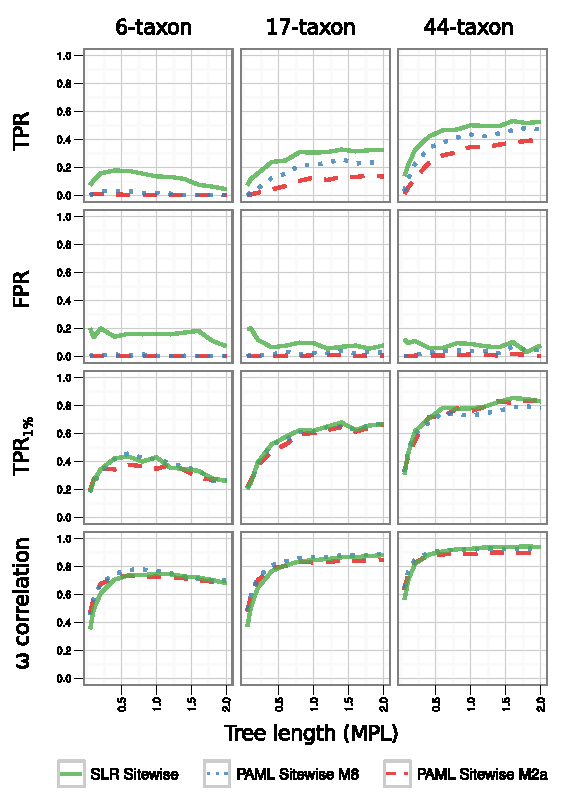
\includegraphics[scale=1]{Figs/fig2.pdf}
\caption{Alignments were simulated without indels for three tree
  shapes and analyzed with SLR, \meight, or \mtwo. Fifty replicate
  alignments were simulated for each data point. The performance of
  each analysis method, as measured by four summary statistics, is
  plotted as a function of the mean path length (MPL) divergence. From
  top to bottom: true positive rate (TPR) at the recommended cutoff
  threshold (0.95 for PAML and 3.84 for SLR); false positive rate
  (FPR) at the recommended cutoff threshold; TPR at a 1\% FPR
  threshold; Pearson's correlation coefficient between the true and
  inferred sitewise \omg.}
\label{fig_2}
\end{figure}

\section{Results and discussion}
\subsection{The performance of three methods for detecting \sw positive selection}
I first evaluated the ability of three \sw methods, \mtwo, \meight
and SLR, to accurately estimate \sw \omg values and to detect
positive selection under a range of tree lengths in the absence of
alignment error. Figure \ref{fig_2} shows the TPR, FPR, \tpr{} and \sw
\omg correlation over a range of mean path lengths
(MPL, defined as the mean root-to-tip branch
  length across all lineages) for each of the three simulation trees.

The detection power and \omg correlation were weakest at low
divergence levels for all methods and all trees due to the low amount
of evolutionary information, as observed in previous simulations
\citep{Anisimova2002}. I found a positive correlation between
tree size and detection power, with the highest performance in the
44-taxon tree. Power generally increased monotonically with
divergence, except for the 6-taxon tree which saw its maximum
performance at moderate divergence levels (MPL 0.5--1.0) and began
decreasing at higher values. The downward trend in the 6-taxon tree
was likely due to the impact of saturation of \syn sites in the
very long branches present in such a sparse tree at high divergence
levels. With lower average branch lengths at equivalent MPLs, the two
larger trees showed no signs of decreased performance even at a MPL of
2 substitutions per site, which is greater than any of the divergence
levels found in groups of commonly analyzed vertebrate, insect and
fungal species (Table \ref{table_2}).

Comparing the three methods for detecting positively selected sites, I found that at the
recommended cutoff threshold (Figure \ref{fig_2}, top row) SLR showed
the highest power to detect positive selection in all trees, followed
by \meight and \mtwo. In the smallest tree, the power of the two
PAML methods was virtually zero while SLR reached a maximum TPR of ~18\%
(at MPL=0.5). At the same divergence, SLR yielded TPRs of 25\% and 45\%
in the 17-taxon and 44-taxon trees, respectively, with \mtwo ranging
between 50--75\% of SLR's power and \meight falling between the two
other methods.

The TPR measurements represent the power that might be achieved in
real-world analysis using recommended cutoff thresholds, but the
higher power from SLR may merely reflect a shifted balance between
power and accuracy at the recommended cutoff threshold as opposed to
an increased absolute ability to discriminate positive from neutral or
purifying selection. The FPR and error-controlled \tpr results
revealed that this was indeed the case: the FPR from SLR was higher
than that from either of the PAML methods for all trees and divergence
levels, suggesting that its higher power was the result of a
less-conservative cutoff value. This was further verified by
evaluating the TPR at a cutoff threshold that controlled for an actual
FPR of 1\% for each method (\tpr{}, third row in Figure
\ref{fig_2}). The error-controlled \tpr values were virtually
identical for all three methods, providing strong evidence that the
three methods' \sw statistics were nearly equally sensitive to
positive selection under the chosen simulation conditions.

The conservative nature of the default thresholds for PAML and SLR has
been previously noted
\citep{Anisimova2002,Yang2005Bayes,Massingham2005}, but the extremely
low false positive rates in these simulations showed that in the
absence of alignment error all three methods would yield very few
false positives when analyzing genes with a typical mammalian-like
distribution of \omg values. The low FPRs were likely due to the large
proportion of sites under moderately strong purifying selection in the
\omg distribution used for simulation. Such sites are less likely to
yield false positives than sites under neutral evolution (\omg$=$1), the
null model against which tests for positive selection are
traditionally controlled.

For the purposes of these indel experiments, the observed similarity in
error-controlled power levels indicated that the behavior of \mtwo,
\meight, and SLR was similar enough not to warrant separately
evaluating all three methods in the subsequent indel simulation
experiments. As the runtime for SLR was significantly lower than that
of either PAML model, all subsequent results are presented only based
on the SLR test.

\subsection{The Effect of Alignment Error on \Sw Power}

When the indel rate was greater than zero, performance levels varied
significantly for different tree sizes, alignment algorithms, and
evolutionary divergences. Figure \ref{fig_3} shows the same
performance measurements as Figure \ref{fig_2} for simulations without
indels (gray lines, Figure \ref{fig_3}) and with indels (black and
textured lines, Figure \ref{fig_3}) analyzed using three different
aligners (ClustalW, MAFFT, and \prankc) and the true
alignment. (Results for ProbCons, T-Coffee and \pranka alignments are
generally of intermediate quality, with ProbCons and T-Coffee showing
slightly higher TPR, slightly higher FPR, and very similar \tpr{}
compared to MAFFT, and \pranka showing performance levels superior to
these but inferior to \prankc. These results are omitted from Figure
\ref{fig_3} in order to reduce visual clutter; \tpr results for
\pranka are shown in Figure \ref{fig_4}C and discussed in the next
section, and a comparison of results from all aligners tested can be
found in Figure \ref{fig_s1}.) For the indel simulations, the indel
rate here was held constant at 0.1 indel event per substitution.

\begin{figure}[t!]
\centering
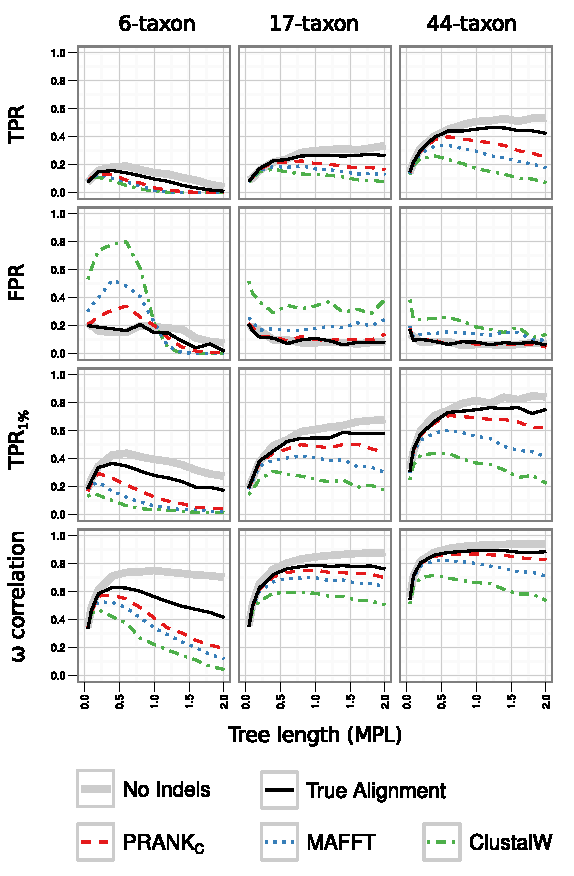
\includegraphics[scale=0.9]{Figs/fig3.pdf}
\caption{Performance of sitewise detection of positive selection with
  alignment error. Sequences were simulated without indels (solid gray
  lines) or with indels (solid black and textured lines) using one of
  three tree shapes, aligned with one of three aligners, and analyzed
  with SLR; true alignments were separately analyzed with SLR (solid
  black lines). One hundred replicate alignments were simulated for
  each data point. The performance of each dataset, as measured by
  four summary statistics, is plotted as a function of the mean path
  length (MPL) divergence. From top to bottom: true positive rate
  (TPR) at the recommended cutoff threshold; false positive rate (FPR)
  at the recommended cutoff threshold; TPR at a 1\% FPR threshold;
  Pearson's correlation coefficient between the true and inferred
  \omg.}
\label{fig_3}
\end{figure}

Comparing the results without indels to those with indels under the
true alignment I found a slight decrease in power and \omg
correlation and no noticeable increase in FPR. The decreased power was
expected, since even in the absence of alignment error alignment
columns containing gaps harbor less evolutionary information than
columns with complete sequence data. The lack of increased FPR showed
that SLR retained its conservative statistical performance even when
analyzing gapped alignments. Surprisingly, at higher divergences (MPL$>$1.0) under the six-taxon tree, the FPR with indels was lower than
the FPR without indels. This unexpected result may be attributed to
the large number of alignment columns under such conditions that
contained only a single non-gap sequence, as those columns were never
inferred as positively-selected by SLR due to the complete lack of
information. The two larger trees did not show a similar trend at high
divergence levels, suggesting that this effect was indeed due to the
highly sparse nature of the alignments in the 6-taxon tree. All other
results from the 6-taxon tree at high divergences were similarly
anomalous in this respect; I surmised that the sparseness of the true
alignment, combined with the extreme difficulty of accurately aligning
sequences along very long branches, made \sw analysis with indels very
unreliable at high divergences in the smallest tree.

When alignments were inferred using one of the three aligners tested,
the TPR, \tpr{} and \omg correlation were all reduced relative to
the true alignment (dashed and dotted lines, Figure \ref{fig_3}). The
degree of reduction varied depending on the aligner, simulation
conditions, and performance measurement being analyzed. At low
divergences (e.g. MPL$<$0.2) the inferred alignments generally
showed only a small decrease in performance. As divergence levels
increased, so did the difference between the performance of the true
alignment and the inferred alignments. The three aligners tested could
be consistently and unambiguously ranked by all of the measured
performance characteristics, with \prankc always performing best and
ClustalW performing worst. The same ranking of aligners with respect
to detecting positive selection has been observed in a number of
studies
\citep{Fletcher2010,MarkovaRaina2011,Privman2011Improving};
my results corroborate these findings and provide evidence that this
ranking may be consistent across a wide range of divergence levels and
indel rates.

Looking at the TPR results for inferred alignments, I observed that
in the 6-taxon tree the three aligners formed a cluster of lines well
below the true alignment value, indicating similar tendencies among
the different aligners to produce false negatives in the smaller
tree. In larger trees the different aligners showed a wider spread of
TPR values, but even \prankc{} showed a 5--10\% reduction compared to
the true alignment at MPL$=$1.0. These results show that the
introduction of false negatives is a significant and seemingly
unavoidable result of alignment error at medium to high divergence
levels (MPL$>$0.5), with even the most successful aligner producing
a marked reduction in TPR compared to the true alignment. The \tpr and
\omg results in the larger two trees were qualitatively similar to
the TPR results, showing that the aligners tested led to different
levels of sitewise performance even when controlling for actual error
rates or assessing the sitewise \omg correlation.

The FPRs for inferred alignments exhibited a very different trend from
the other performance measures, with generally higher FPRs than the
true alignment and the widest range of values occurring in the 6-taxon
tree. In this tree at medium divergence levels (e.g.\, MPL$=$0.2--0.6)
ClustalW showed up to a fourfold increase, and \prankc{} a nearly
twofold increase, in FPR over the true alignment. As previously noted,
the 6-taxon tree showed an anomalous FPR pattern at higher
divergences, with lower FPRs for inferred alignments than the true
alignment, likely due to the highly sparse true alignment under those
conditions. In the two larger trees, FPRs from inferred alignments
were less elevated compared to the true alignment, less variable
between aligners, and relatively constant across the range of
divergences. ClustalW's FPR ranged between 0.001 to 0.005, while
\prankc{}'s FPR was virtually identical to that of the true alignment
in the 17-taxon and 44-taxon trees.

%% I found it useful to combine divergence estimates from Table
%% \ref{table_2} with the results from Figure \ref{fig_3} to characterize
%% the combined effects of alignment error at different commonly analyzed
%% levels of divergence. For example, at a human-mouse divergence level
%% (MPL$=$0.2) misalignment had little impact on the TPR regardless of
%% what aligner was used. However, ClustalW yielded a notably higher FPR
%% than MAFFT or \prankc, and the error-controlled \tpr{} was
%% correspondingly lower for ClustalW in all three trees. Thus, at low
%% divergences I found that false positives were the main source of
%% error from misalignment, and different aligners had highly variable
%% tendencies to produce false positive results. At higher vertebrate and
%% \Dr divergence levels (MPL$=$0.8--1.0) false negatives became much
%% more prevalent. The TPR for all inferred alignments was virtually zero
%% in the 6-taxon tree, underscoring the necessity of including many
%% species in the analysis of highly diverged sequences. In the two
%% larger trees, \prankc resulted in very few additional false positives,
%% but it suffered a 5--10\% reduction in TPR relative to the true
%% alignment. Meanwhile, ClustalW showed a 50\% TPR reduction and
%% maintained a strongly elevated FPR. At higher divergences and in
%% larger trees, false negatives were thus the most persistent effect of
%% alignment error, causing a marked reduction in \sw power even with the
%% best-performing aligner. Overall, the ranking of aligners was clear,
%% with \prankc performing better than MAFFT and MAFFT performing better
%% than ClustalW across all performance measures and MPL divergence
%% levels.

\begin{figure}[t!]
\centering
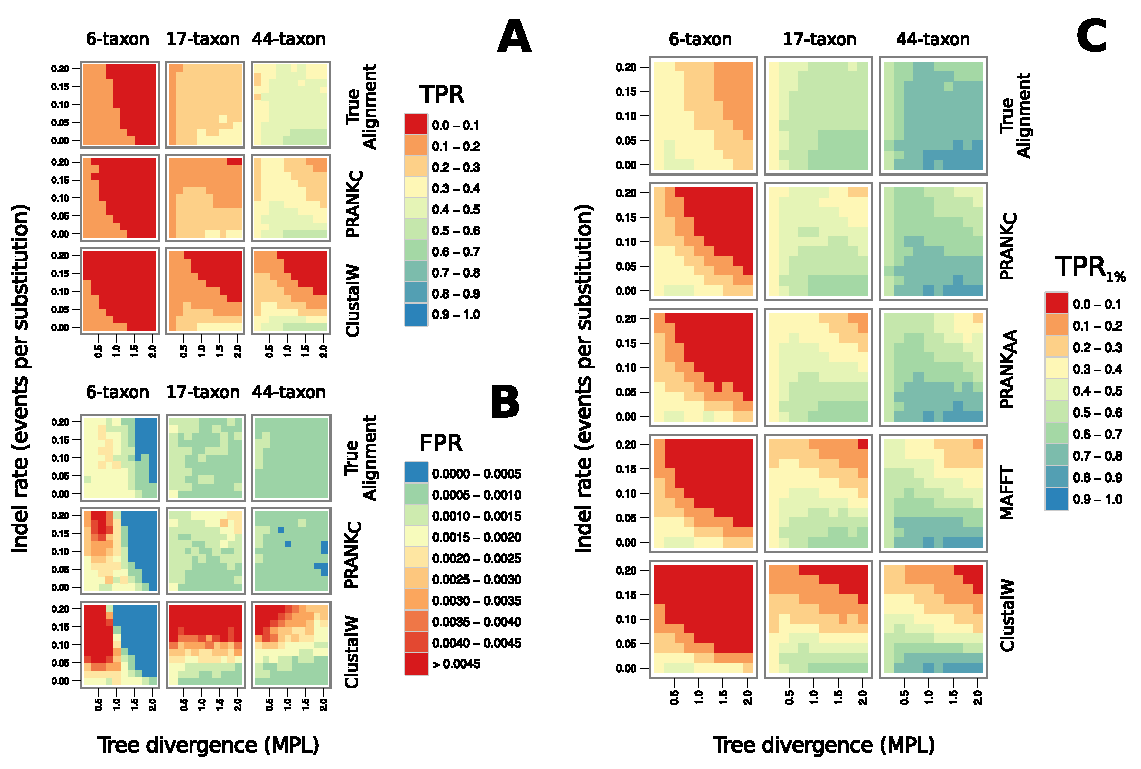
\includegraphics[scale=0.8]{Figs/fig4.pdf}
\caption{The TPR, FPR, and \tpr for \sw detection of positive
  selection. Sequences were simulated with indels using one of three
  tree shapes (6-, 17- or 44-taxon) and a range of indel rates and
  mean path length (MPL) divergence levels. Alignments are inferred
  with one of four aligners (ClustalW, MAFFT, \pranka{}, \prankc) and
  analyzed with SLR; true alignments were separately analyzed with
  SLR. One hundred replicates were simulated for each set of
  conditions. Each cell is colored according to the performance at a
  given (indel rate, MPL) pair as measured by one of three summary
  statistics: (A) the true positive rate (TPR) at the recommended
  cutoff threshold, (B) the false positive rate (FPR) at the
  recommended cutoff threshold, or (C) the TPR at a 1\% FPR
  threshold. Results for MAFFT and \pranka are omitted from (A) and
  (B); as in (C) they show characteristics intermediate between
  ClustalW and \prankc.}
\label{fig_4}
\end{figure}

\subsection{\Sw Power Under a Range of Indel Rates and Divergences}

To explore the effects of alignment error across a wider range of
simulation conditions, I extended the simulations of Figure
\ref{fig_3} across multiple indel rates. Figure \ref{fig_4} shows
heatmaps of the TPR and FPR for ClustalW, \prankc and the true
alignment (Figure \ref{fig_4}A, B) and a heatmap of the
error-controlled \tpr for all aligners tested (Figure \ref{fig_4}C).
(MAFFT and \pranka are omitted from Figure \ref{fig_4}A, B and
ProbCons and T-Coffee are entirely omitted from Figure \ref{fig_4} for
clarity. The performance of all these aligners fell between that of
ClustalW and \prankc for all measurements. \pranka slightly
outperformed MAFFT, and ProbCons and T-Coffee showed similar
performance to MAFFT. A comprehensive set of TPR, FPR, and \tpr
results can be found in Figure \ref{fig_s1}.) The results from Figure
\ref{fig_3}, which were simulated with an indel rate of 0.1,
correspond to the middle row of each panel in Figure \ref{fig_4}; rows
above and below the middle row represent higher and lower indel rates,
respectively. Similarly, the bottom row of each panel in Figure
\ref{fig_4} was simulated with an indel rate of zero and corresponds
to the `No Indels' data in Figure \ref{fig_3}.

The TPR values (Figure \ref{fig_4}A) show a consistent pattern
across the range of indel rates, with power decreasing as either the
indel rate or the divergence level increases (except at the lowest
divergence levels, where the lack of evolutionary information yielded
slightly lower TPRs in the larger two trees). \prankc{} showed a
greater ability than ClustalW to maintain a high TPR at higher indel
rates, especially in the 17-taxon and 44-taxon trees. At lower indel
rates, the TPR performance of both aligners and the true alignment
were qualitatively similar.

\prankc{} and ClustalW both showed a qualitatively similar pattern of
elevated FPRs in the 6-taxon tree (Figure \ref{fig_4}B), but their
behavior diverged significantly in the 17-taxon and 44-taxon trees. In
the 17-taxon tree, \prankc{} only showed an elevated FPR compared to
the true alignment at very high indel rates and divergence levels, but
the ClustalW FPR increased steadily with the indel rate, quadrupling
in value from the lowest to highest indel rate. Interestingly, for any
given indel rate, the ClustalW FPR showed little variation across the
range of divergence levels. This result was counter-intuitive, as we
expected alignment errors to become more common as divergence
increased and the number of observed indel events grew. Furthermore,
\prankc{} behaved as expected, showing increased
FPRs only at the highest divergences and indel rates in the 17-taxon
tree. The FPR results in the 44-taxon tree confirmed the strange
effect of ClustalW's alignments on the \sw FPR: at the highest indel
rates, ClustalW showed a negative relationship between FPR and
divergence---exactly opposite to the trend I expected. \prankc{}'s
FPR in the 44-taxon tree was equal to or below that of the true
alignment under almost all conditions.

The error-controlled \tpr results (Figure \ref{fig_4}C) provide a
comprehensive picture of the effect of alignment error on the detection of
\sw positive selection. The two aligners not shown in the two other
panels (MAFFT and \pranka) exhibited \tpr values intermediate to those
from ClustalW and \prankc across the range of parameters tested, with \pranka performing
better than MAFFT. As
expected, performance was very similar between aligners at very low
indel rates. At higher indel rates, most aligners yielded similar
patterns of low \tpr in the 6-taxon tree, but in the larger two trees
ClustalW and MAFFT alignments were unable to achieve high \tpr
values, presumably due largely to their elevated FPR in those trees.

It is worth noting the ability of \prankc to maintain a very low level
of false positive sites even under extremely difficult alignment
conditions. Although \prankc showed slightly elevated FPRs at high
indel rates in the 17-taxon tree, FPRs were nearly identical to the
true alignment across all simulated conditions in the 44-taxon
tree. This impressive performance suggests that, given a large enough
number of taxa, \prankc alignments would yield very few erroneous
false positives in scans for positive selection in sequences with even
very high divergence levels. Furthermore, these results showed that
false negatives contributed more than false positives to \prankc{}'s
reduction in \sw performance---a novel observation which provides
insight into the nature of \prankc alignments and their application to
\sw evolutionary analysis.

\begin{landscape}
\begin{figure}
\centering
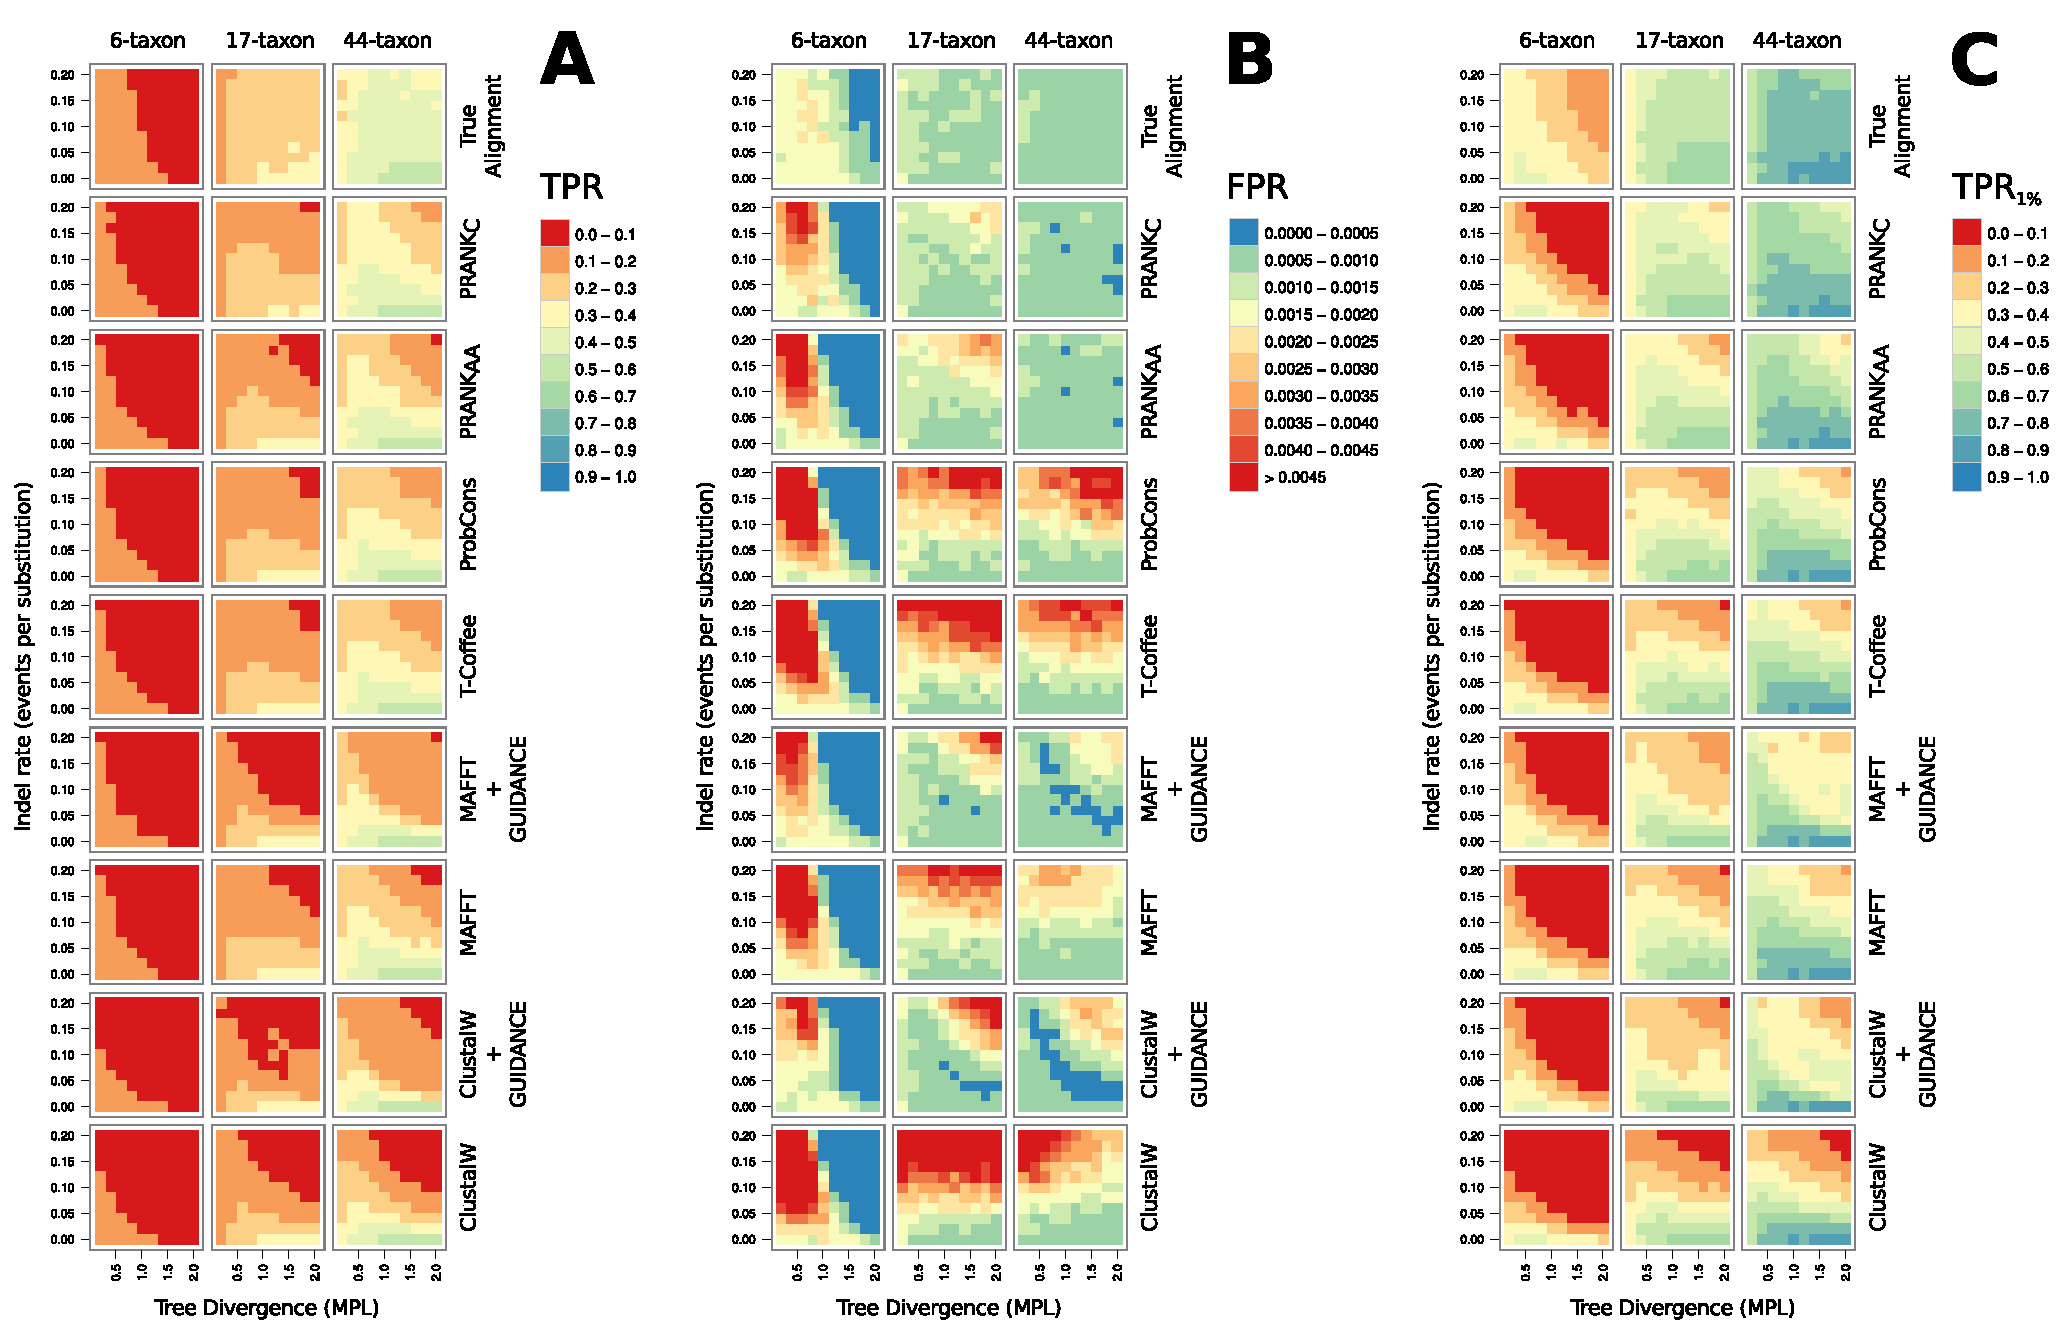
\includegraphics[scale=0.65]{Figs/supp_fig1.pdf}
\caption{This figure depicts the same simulations and uses the same
  formatting as Figure 4, except that results for MAFFT and \pranka
  have been added to sections (A) and (B) and results using ProbCons,
  T-Coffee, ClustalW + GUIDANCE, and MAFFT + GUIDANCE have been added
  to all sections.}
\label{fig_s1}
\end{figure}
\end{landscape}

\subsection{Effect of Alignment Filtering on \Sw Error Rates}

\begin{figure}[t!]
\centering
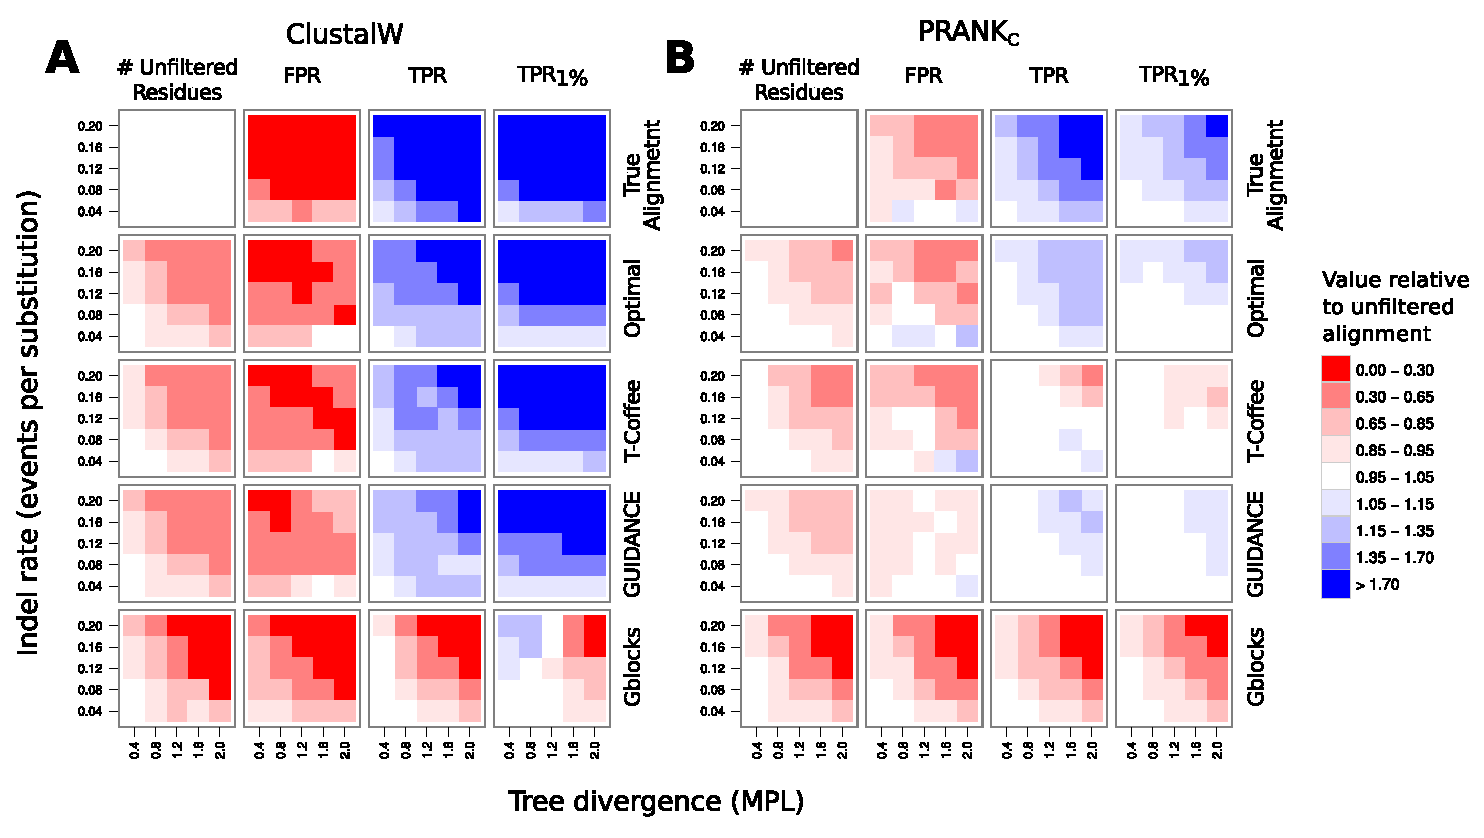
\includegraphics[scale=0.65]{Figs/fig5.pdf}
\caption{The effect of alignment filtering on sitewise detection of
  positive selection. Sequences were simulated using the 17-taxon tree
  and a range of indel rates and mean path length (MPL) divergence
  levels. Alignments were inferred using (A) ClustalW or (B) \prankc,
  either left unfiltered or filtered with one of four alignment
  filters (Optimal, T-Coffee, GUIDANCE, Gblocks), and analyzed with
  SLR; true alignments were left unfiltered and separately analyzed
  with SLR. One hundred and fifty replicates were simulated for each
  set of conditions. Cells are colored according to the ratio of the
  performance of the indicated filter to the performance of the
  unfiltered ClustalW or \prankc alignment as measured by one of four
  summary statistics. In columns from left to right: the number of
  unfiltered (i.e., non-$N$) residues remaining in the alignment; the
  false positive rate (FPR) at the recommended cutoff threshold; the
  true positive rate (TPR) at the recommended cutoff threshold; the
  TPR at a 1\% FPR threshold (\tpr). Note that the maximum percentage
  of residues removed by filtering was capped at 50\% for all methods
  except Gblocks.}
\label{fig_5}
\end{figure}

Having established that alignment error can lead to reduced \sw
performance through the introduction of false negatives and false
positives, I tested whether alignment filtering methods could reduce
error rates and improve the power of \sw detection of positive
selection. Using sequences simulated from the 17-taxon tree and a
range of indel rates and divergence levels, I calculated inferred
alignments using ClustalW and \prankc and applied four filtering
methods before performing the \sw analysis. Since I wished to
determine whether alignment filters either improved or worsened the
error rates and power of \sw analysis, I measured the ratio of each
performance measure to the value obtained from the equivalent
unfiltered alignments. These relative values are presented in Figure
\ref{fig_5}. (Filtering results for \pranka, ProbCons and
  T-Coffee were not calculated, and results for MAFFT are omitted from
  Figure \ref{fig_5} to save space. The gain or loss in performance
  resulting from filtering MAFFT alignments was generally intermediate
  to that resulting from filtering ClustalW or \prankc alignments. A
  comprehensive set of filtering results, including MAFFT alignments
  and \tprf values, can be found in Figure \ref{fig_s2}.)

As alignment filters act through the removal of alignment residues or
columns, a certain amount of reduction in both the FPR and TPR was expected
purely from the decreased amount of information available. For
example, a filter that randomly removes a fraction of residues of each
alignment would be expected to produce equal reductions in FPR and
TPR. A more effective filter may also yield a reduced TPR, but the FPR
reduction would be larger in magnitude, making the detection of
positive selection more powerful for a given error rate. Thus, a
reduced FPR is not necessarily indicative of good filtering
performance, nor is a reduced TPR necessarily indicative of poor
filtering performance. Additionally, the prevalence of false negatives
resulting from misalignment suggested the interesting possibility that alignment filters may also
improve power by removing false negatives, perhaps by masking out
residues that were preventing positive sites from being
identified. The removal of false negatives would result in an
increased TPR, further complicating the assessment of filtering
results based on FPR or TPR alone. As a result, I focused on the
change in error-controlled \tpr{} as the best single measure of
whether a filter had successfully improved the \sw power of a dataset
since this value is sensitive to changes in both the FPR and TPR. Note
that the \tpr controls the FPR post-filtering, accounting for the
tendency of filtering to reduce the FPR at a given cutoff threshold.

I first examined the two controls, the unfiltered true alignment and
the inferred alignments filtered with the optimal filter (top two
rows, Figure \ref{fig_5}). The true alignment nearly always showed
smaller FPR (red cells) and greater TPR and \tpr (blue cells) compared
to the inferred alignments, with a greater magnitude of change
relative to the ClustalW alignments than to the \prankc alignments
(darker shades cf. lighter shades). These scores represented the
direction and an upper limit on the magnitude of change that might be
achieved by a perfect alignment filter. One exception to the general
trend of lower FPR in the true alignment was the observation of two
simulation conditions with slightly elevated FPRs in the true
alignment compared to \prankc alignments (at an indel rate of 0.04 and
MPL of 0.8 and 2.0). This small inconsistency may be explained by
stochastic variation in false positive counts, as the absolute value
of the FPR was very low in both datasets under those
conditions. Figure \ref{fig_4}B shows the FPR to be on the order of
$5\times10^{-4}$ under those conditions; in total, I observed 63
false positives for the true alignment and 67 false positives for the
\prankc alignment at the indel rate of 0.04 and MPL of 0.8 across all
150 replicates (comprising ca.\ 75,000 analyzed sites). A similar
slight FPR elevation was also observed at the same indel rate for the
optimal, GUIDANCE and T-Coffee filters.

\begin{landscape}
\begin{figure}
\centering
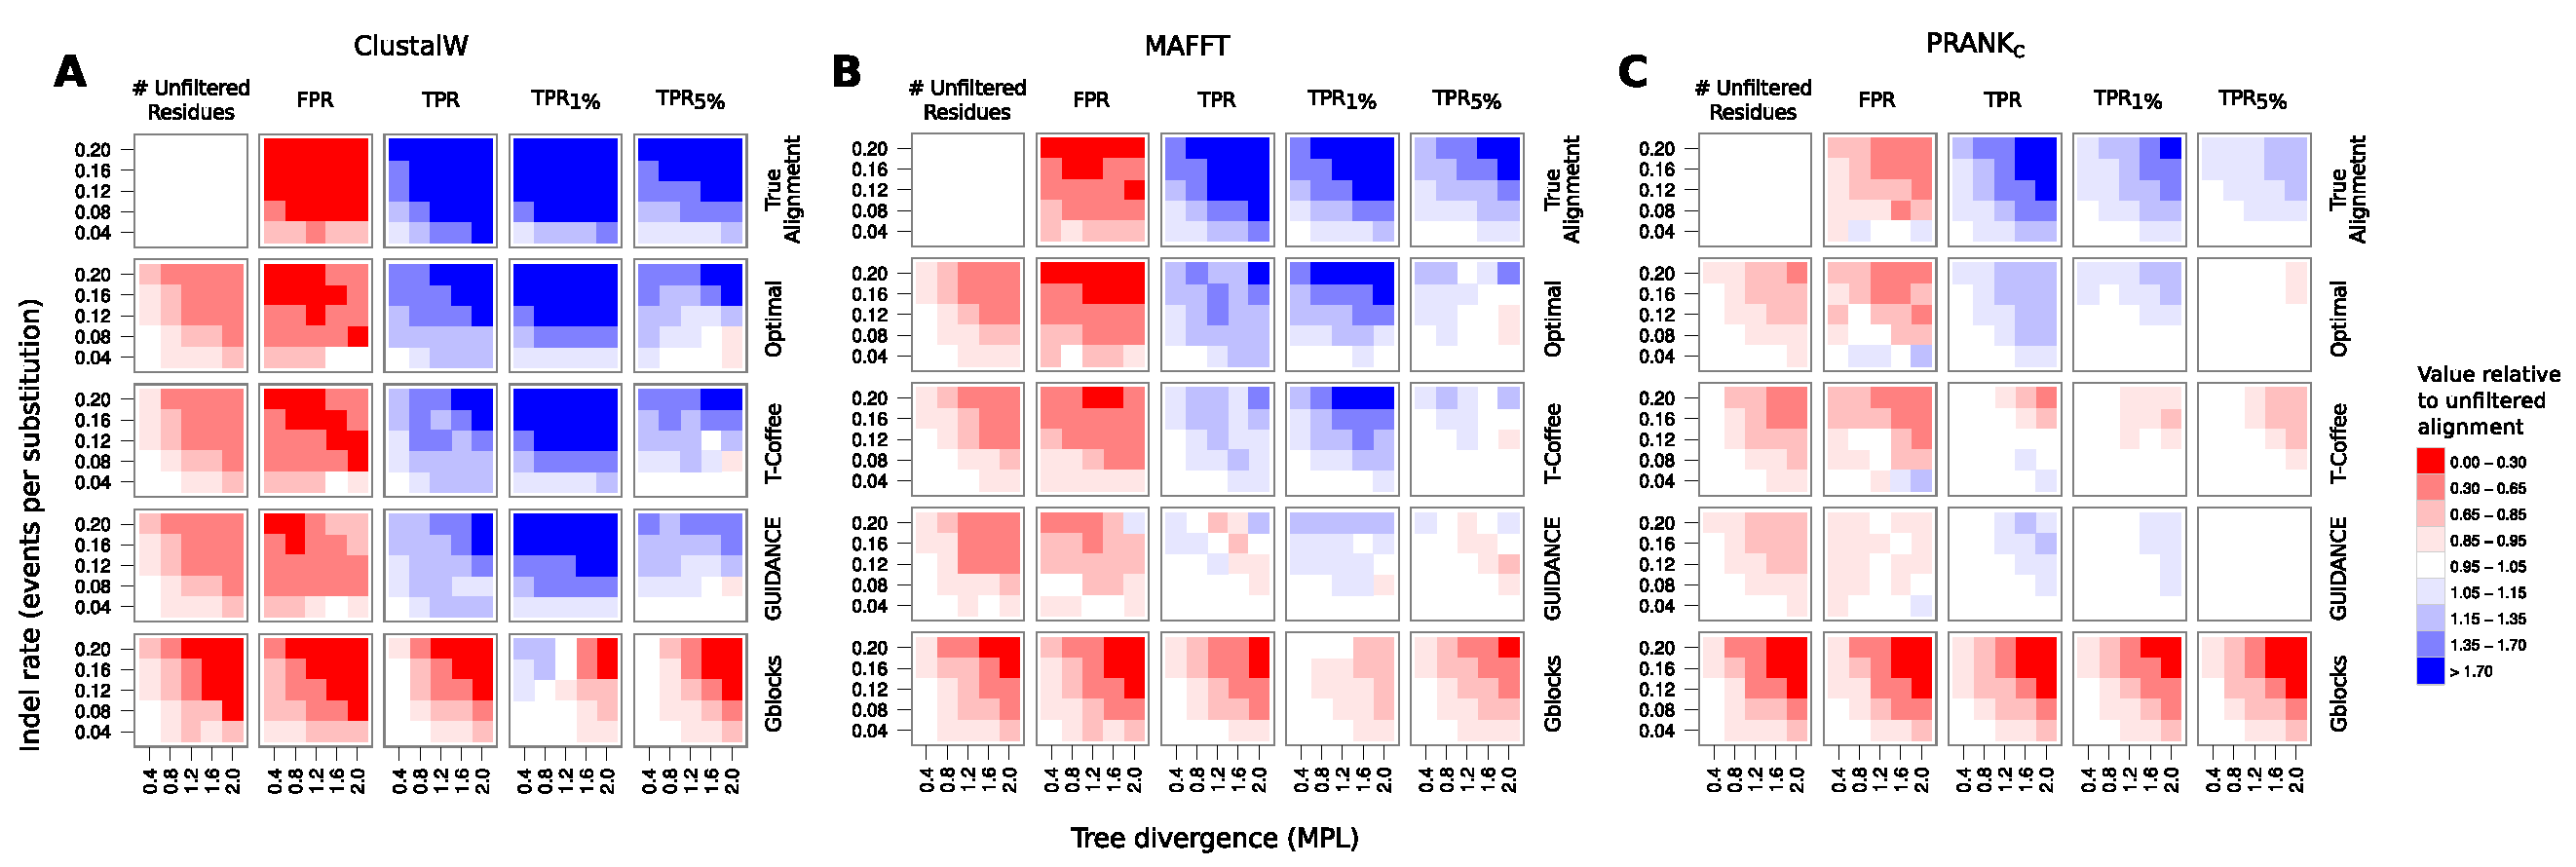
\includegraphics[scale=0.55]{Figs/supp_fig2.pdf}
\caption{This figure depicts largely the same simulations and uses the
  same formatting as Figure 5 except for two changes. First,
  results for MAFFT have been added to section (B) and results for
  \prankc have been moved to section (C). Second, the rightmost column
  has been added, showing the true positive rate (TPR) at a 5\% false
  positive rate (FPR) threshold (labeled \tprf).}
\label{fig_s2}
\end{figure}
\end{landscape}

The expectation was that the optimal filter would show the same
direction of change in FPR and TPR as the true alignment, but with
slightly lower magnitudes. Indeed, improved \sw performance was
achieved in nearly all simulation conditions by the optimal filter,
with the magnitude of \tpr change slightly lower than for true
alignment. For ClustalW alignments the amount of improvement was quite
large, with $>$70\% increase in \tpr for nearly all conditions with an
indel rate above 0.1. The improvement was more modest for \prankc
alignments with a maximum of 15--35\% \tpr increase.

Looking at the reduction in the number of non-masked residues
remaining after filtering, I found that the optimal filter reached
the maximum of 50\% filtered residues for all ClustalW alignments with
MPL$>$1 and an indel rate$>$0.1. This meant that more than 50\% of
residues were correctly aligned across less than 50\% of the tree in
those alignments. By contrast, the optimal filter applied to \prankc
alignments only reached the maximum of 50\% filtered residues at the
highest tested divergence level and indel rate combination.

The TPR improvements achieved by the optimal filter provided some
insight into the nature of sitewise false negatives resulting from
alignment error. Two different types of alignment error might cause a
false negative at a positively-selected site: either misalignment of
one or more \nh codons causing the positive signal to be
masked, or non-alignment of homologous codons causing the amount of
evolutionary information to be reduced. The former type of error would
be recoverable by alignment filtering (through removal of the codon(s)
masking the positive signal), but the latter would not. Thus, the
ability of the optimal filter to improve TPR levels across the board
provided evidence that a sizeable portion of false negatives from both
ClustalW and \prankc alignments were due to misaligned codons and thus
amenable to recovery by filtering. Although the optimal filter was
unrealistic in that it was based on perfect knowledge of which codons
were misaligned, this result provided hope that one of the other
filters might show a similar ability to recover false negative errors
from \prankc alignments.

Turning to the three filters under investigation, I found T-Coffee
and GUIDANCE both to be highly effective at improving ClustalW
alignments, with magnitudes of improvement near those of the optimal
filter. When applied to \prankc alignments, however, the two filters'
behavior diverged: T-Coffee only showed unchanged or reduced \tpr, but
GUIDANCE yielded slightly improved \tpr at high divergence levels and
indel rates, with values 5--15\% greater than the unfiltered \prankc
alignments. Both filters removed similar amounts of sequence
information and resulted in similarly reduced FPR levels, but GUIDANCE
showed a unique ability to recover false negatives from \prankc
alignments at the highest divergence levels and indel rates, and the
resulting TPR elevation appears to have been responsible for the
increased \tpr performance.

Gblocks behaved very differently from the other filters tested,
resulting in reduced FPR, TPR, and \tpr under nearly all simulation
conditions. Only at high indel rates and low divergence levels in the
ClustalW alignments did Gblocks show increased \tpr relative to the
unfiltered alignments. This poor performance was likely due to
overly-aggressive removal of alignment columns. I could not limit the
amount of sequence masked by Gblocks, so many alignments saw more than
70\% of residues removed, resulting in the loss of a large number of
correctly-aligned true positive
sites. \citet{Dessimoz2010Phylogenetic} found Gblocks filtering to
have a negative effect on the accuracy of phylogenetic inference; the
current results provide additional evidence in support of their
finding, suggesting that Gblocks filtering tends to reduce, rather
than increase, the power and accuracy of alignments when applied to a
number of evolutionary analyses.

There was some evidence that the column-wise nature of Gblocks
filtering was partly responsible for its poor performance here. Since
false negative errors cannot be recovered through the removal of
entire alignment columns, it made sense that the \prankc
alignments---which resulted in varying numbers of false negatives but
always very few false positives---would not see improved performance
after column-wise filtering. On the other hand, ClustalW alignments
showed a relatively constant level of false positives and an
increasing number of false negatives as divergence levels
increased. The application of a column-wise filter like Gblocks would
thus be expected to show good improvement at low divergences where
false positives dominated, but less improvement at higher divergences
where false negatives became more prominent. Indeed, this was the
pattern observed when applying Gblocks to ClustalW alignments.

Overall, the alignment filtering simulations found that Gblocks rarely
improves alignments for sitewise detection of positive selection, but
filtering methods based on {GUIDANCE} and T-Coffee scores have a good
ability to mask out misaligned residues that cause false positives and
false negatives in sitewise inference. This beneficial effect was
highly dependent on simulation conditions and the input aligner. For
ClustalW alignments (which, left unfiltered, led to many false
positives and false negatives) both GUIDANCE and T-Coffee showed good
ability to improve sitewise performance, behaving qualitatively
similarly to the optimal filter.

Since the performance measurements shown in Figure \ref{fig_5} are
expressed relative to values obtained with unfiltered alignments, they
do not allow for easy comparison of the absolute performance of any
combination of aligner and filter. To more directly compare the
absolute TPR, FPR and \tpr values obtained with filtered ClustalW and
MAFFT alignments to those obtained with other unfiltered alignments, I
simulated additional datasets with ClustalW and MAFFT alignments and
GUIDANCE filtering using all three trees and the same range of indel
rates and MPLs as used for Figure \ref{fig_4}. These results are
included in Figure \ref{fig_s1}. Comparing absolute performance, I
found that GUIDANCE filtering generally improved the \tpr for ClustalW
and MAFFT alignments, largely due to strong FPR reductions in regions
of high indel rates and low divergence levels. The resulting \tpr
performance for filtered ClustalW alignments was comparable to (but
not better than) unfiltered MAFFT alignments, and the \tpr for
filtered MAFFT alignments was slightly better than unfiltered MAFFT
alignments and substantially worse than unfiltered \pranka alignments.


Filtering was less beneficial when applied to the more accurate
\prankc alignments, with T-Coffee filtering reducing performance and
GUIDANCE yielding only mild \tpr improvements. Importantly, GUIDANCE
only showed improved performance at high divergence levels (e.g.,
MPL$>$1.6), well above those found in commonly-analyzed groups of
species. Thus, the use of unfiltered \prankc alignments would yield
largely equivalent performance to GUIDANCE-filtered alignments for
detecting \sw positive selection when analyzing protein-coding
sequences at most commonly encountered divergence levels. Equally
important was the observation that GUIDANCE (when judiciously applied,
including an upper limit on the amount of sequence data removed) did
not significantly reduce performance compared to the unfiltered
alignments. Put simply, filtering neither significantly hurt nor
significantly improved performance. Finally, it should be noted that
the performance of the `optimal' filter on \prankc alignments suggests
that mild further improvements to filtering strategies may be
possible; however, the potential for improvement is small and may be
of little practical value.

\section{Conclusions}

In this chapter, I investigated the performance of sitewise detection
of positive selection under a range of tree sizes, indel rates, and
divergence levels, using simulation parameters designed to approximate
the analysis of typical mammalian protein-coding genes. I evaluated
the ability of six alignment methods and three alignment filtering
methods to produce alignments for detecting positively selected sites,
using the FPR, TPR, and error-controlled \tpr of the sitewise
detection of positive selection as measures of performance.

The simulation results showed that alignment error can have a
measurable impact on the error rates and power of the sitewise
detection of positive selection under all but the least difficult
alignment conditions. I confirmed and extended the findings of
\citet{Fletcher2010}, \citet{MarkovaRaina2011}, and
\citet{Privman2011Improving} regarding the relative accuracy of
different aligners, showing that \prankc had the best performance and
ClustalW had the worst performance for subsequent sitewise
analysis. Notably, these simulations found that ClustalW produced more
sitewise false positives than any other aligner tested even at low
divergence levels, suggesting that its use should be avoided even when
analyzing closely-related sequences. \prankc, on the other hand,
resulted in very low FPRs even at higher divergences. In particular,
when the number of sequences in the tree was large, \prankc{}'s
sitewise FPRs were virtually indistinguishable from those of the true
alignment.

An important observation regarding the size of tree analyzed was that
the 6-taxon tree caused qualitatively similar problems (e.g.\,
elevated FPRs and reduced TPRs) for all aligners, suggesting that poor
performance is inevitable when analyzing a small number of moderately
divergent sequences. The small amount of evolutionary information
combined with the longer branch lengths makes alignment difficult and
increases the tendency of misalignment to cause sitewise false
positives. Thus, I reiterate the well-established recommendation to
use large numbers of sequences when inferring sitewise positive
selection \citep{Anisimova2001,Anisimova2002}. When analyzing
sequences with indels, the shape of the tree may matter as well: trees
with long internal branches may be especially prone to false
positives, as longer branches are more difficult to align.

The very low FPRs observed for \prankc alignments conflicted somewhat
with the results of \citet{Fletcher2010}, who found that the FPRs for
the branch-site test were not under control even with \prankc
alignments. This apparent discrepancy can be explained by different
sensitivities to alignment error: the branch-site test would yield
false positives when misalignment causes apparent positive selection
along only the foreground branch, while the SLR test would produce
false positives only when misalignment causes a signal of positive
selection strong enough to overpower the non-positive signal
throughout the tree. This effect stems from the different biological
hypotheses tested by the two methods; their differential sensitivity
to misalignment underscores the necessity of considering the
biological sensitivity and robustness to alignment error when applying
either of these tests to detect positive selection within an
alignment. For the detection of positive selection in highly divergent
or indel-prone sequences, the use of sitewise models instead of the
branch-site test may be a sensible alternative, sacrificing some
sensitivity for better control of false positives.

Despite producing very low FPRs, \prankc alignments still resulted in
an increased number of false negatives compared to the true
alignment. I showed that some of these false negatives were possible
to recover as true positives through alignment filtering, and I found
that both the `optimal' filter and GUIDANCE were able to successfully
recover these false negatives at high divergence levels, resulting in
small but measurable performance improvements over the unfiltered
\prankc alignments.

The manual or automated adjustment of alignments has been thought by
many to be an important step in evolutionary analyses due to fear of a
high prevalence of misalignment-induced false positives. While this is
true for some aligners, this chapter showed that more accurate
alignment algorithms result in significantly fewer false positives in
the subsequent detection of sitewise positive selection. This strongly
reduces the beneficial effect of alignment filtering, so much so that
current filtering methods are scarcely able to improve the performance
of \prankc alignments when analyzed with SLR.

As a result, the use of alignment filtering in the detection of
sitewise positive selection cannot be uniquivocally recommended,
except perhaps for the most divergent and indel-prone
sequences. Importantly, sequences with these levels of divergence are
unlikely to be encountered in analyses focusing on mammalian or
vertebrate genes. Although GUIDANCE showed some ability to improve the
error-controlled power under difficult alignment conditions at high
divergence levels (whereas T-Coffee and Gblocks filtering failed to
improve upon any \prankc alignments), this improvement was modest in
magnitude and was achieved largely through the recovery of false
negatives as opposed to the elimination of false positives. For an
analysis where the control of false positives is the primary concern,
the added computational expense of running many bootstrap alignment
replicates (as performed by GUIDANCE) may not be offset by the
possibility of a slight increase in power. However, GUIDANCE never
significantly reduced power, so its use would not be expected to yield
worse results.

Some of the current conclusions differ from those of
\citet{Privman2011Improving}, who found strong improvements in
error-controlled power by filtering alignments in simulations focused
on three HIV-1 genes. Although the phylogenetic trees they used to
guide their simulations contained divergence levels at the low end of
the range tested here (MPLs of 0.38, 0.34 and 0.33 for gag, pol and
env, respectively; E. Privman, personal communication) and were
roughly comparable in size and shape to the 17-taxon tree, I failed to
find a significant benefit for alignment filters at any MPL below 1.2
when using \prankc alignments. Interestingly, the authors also found
Gblocks to be roughly comparable in performance to GUIDANCE, while I
found Gblocks' performance to be very poor. Some of these
discrepancies may be due to differences in the details of the
simulations or filtering procedures, but in the end the results are
largely complementary: \citet{Privman2011Improving} showed that
filtering can be beneficial for detecting positive selection,
especially in the case of fast-evolving (but fairly closely-related)
sequences, while I have shown that divergence levels and indel rates
have a significant impact on the performance of different aligners and
filters.

It is important to note that the current simulations did not include
fully biologically realistic models of spatial or temporal variability
in the rate of indel formation or in the distribution of selective
pressures (e.g.\, \citet{Whelan2008}). Such heterogeneity should not
affect the main conclusions regarding the relative performance of
different aligners and filters: the trends I observed were consistent
across a wide range of parameter values and tree sizes, suggesting
that they reflect fundamental differences in each method's ability to
align or filter sequences as opposed to artifacts due to the relative
simplicity of the framework introduced here.

However, such heterogeneity is clearly important to the evolution of
mammalian proteins \citep{Fay2003}. Many proteins contain combinations
of structured domains and unstructured regions along their length,
resulting in a discontinuous mix of different structure- and
function-related evolutionary pressures. False positives may be more
prominent in small unconstrained regions, raising FPR levels above
those predicted by simulations with a uniform pattern of
evolution. Functional differences between genes may also influence the
\omg distribution, with some genes or domains showing fewer or more
neutrally-evolving sites than modeled here, making false positive
results either less or more likely, respectively. As such, the
appropriateness of any simulation scheme should be critically
considered when evaluating specific power and error rate estimates in
the context of real-world data analysis.

%% In the case of a protein evolving with a mix of insertion and deletion
%% rates, the current results based on uniform rates could be used to
%% identify tentative upper and lower bounds for the overall error
%% rate. For example, if a small region of a protein is evolving with
%% higher divergence and indel rates than the rest, then the error rates
%% within the less-constrained region should be comparable to these
%% results based on proteins with uniformly high divergence and indel
%% rate. Correspondingly, the overall error rate for the protein would
%% fall somewhere between those observed in the simulations corresponding
%% to the least difficult and most difficult regions of the
%% alignment. Critical to such an analysis is the accurate estimation of
%% the local indel rate, for which a number of methods are currently
%% available or under development
%% \citep{Holmes2005,Cartwright2009Problems}.

%% Species-level differences may also have an effect on error rates in
%% detecting positive selection, as the efficacy of natural selection is
%% highly dependent on effective population size
%% \citep{Ellegren2009}. For example, proteins evolving in \Dr
%% species with a high effective population size should experience
%% stronger positive and purifying selection than in mammals, potentially
%% leading to increased power and reduced error rates when compared to
%% the current simulations based on a mammalian-like \omg distribution.

%% A tangential but interesting observation from these simulations was
%% that all three methods tested in this chapter for the sitewise
%% detection of positive selection were highly conservative when
%% analyzing alignments with a mammalian-like \omg distribution. SLR, for
%% example, yielded FPRs well below the nominal 5\% level. This was due
%% to a mismatch between SLR's null model of neutral evolution
%% ($\omega=1$) and the more realistic distribution of non-positive sites
%% used for simulation (where $\bar{\omega}=0.277$). While the ability of
%% SLR and PAML's sitewise models to distinguish between neutral
%% evolution and positive selection in a well-controlled manner is
%% important, the majority of protein sites tend to evolve under moderate
%% purifying selection. Future work on methods to adaptively adjust the
%% cutoff thresholds to achieve better statistical control under
%% non-neutral (and possibly unknown) \omg distributions could yield much
%% greater power to detect positive selection while maintaining good
%% control of error rates.

I showed here that even relatively simple evolutionary simulation
experiments could sensitively assess the performance characteristics
of different aligners, provide quantitative insight into the practical
effects of alignment error, and suggest areas for future development
of alignment and filtering methods. In the future, I expect the
development of more realistic simulations for protein
evolution---perhaps incorporating structurally-motivated and
empirically validated models of mutation, indel formation and
constraint---to further increase the applicability and accuracy of
such experiments, and I believe that flexible and accessible
simulation programs such as INDELible \citep{Fletcher2009INDELible}
and PhyloSim \citep{Sipos2011PhyloSim} will play an important role in
the quantitative assessment of alignment algorithms and
alignment-dependent comparative analyses.

As genomes rapidly accumulate in the databases and large-scale
analyses become the norm, I hope that the development and application
of alignment methods, which are arguably the most important step in
any evolutionary analysis, will be based on a rigorous understanding
of their behavior and performance when applied to a wide variety of
evolutionary analyses.
